\documentclass[10pt]{iopart}
\usepackage[utf8]{inputenc}
\usepackage[T1]{fontenc}
\usepackage{gensymb}

\usepackage[
maxbibnames=99,
maxcitenames=2,
uniquelist=false,
uniquename=false,
backend=biber,
style=authoryear,
doi=false,isbn=false,url=false
]{biblatex}
\addbibresource{references.bib}
\AtEveryBibitem{%
  \clearlist{language}%
}

% Keywords command
\providecommand{\keywords}[1]
{
  \small	
  \textbf{\textit{Keywords---}} #1
}

\usepackage{mathtools}

%\DeclarePairedDelimiterX{\infdivx}[2]{(}{)}{%
%  #1\;\delimsize\|\;#2%
%}
%\newcommand{\infdiv}{D\infdivx}
%\DeclarePairedDelimiter{\norm}{\lVert}{\rVert}


\begin{document}

\title{Hydroclimate variability structured social interaction in the prehistoric American Southwest}

\author{Nicolas Gauthier$^1$}

\address{$^1$ School of Human Evolution and Social Change, 900 S Cady Mall, Tempe, USA}

\ead{Nicolas.Gauthier@asu.edu}

\begin{abstract}
  Do small-scale farmers prefer to interact with others experiencing different weather patterns? In agricultural societies, farmers use their social networks to absorb the impacts of droughts and floods by facilitating resource flows to affected settlements and population flows away from them. These benefits depend on the degree to which a social network connects populations in topographically accessible locations that tend to experience different weather patterns. The patterns by which droughts covary in space and time thus ought to interact with patterns of landscape connectivity to structure prehistoric social networks. Here I use an empirical archaeological case study from the late pre-Hispanic period in the North American Southwest to examine the relationship between drought variability and human social networks over the long term. I analyze 7.5 million artifacts collected from nearly 500 archaeological sites, and estimate how the flow of social information between sites varied as a function of distance and growing-season aridity. I find that although the intensity of social interaction in the past was highly distance dependent, interaction between regions experiencing different domains of externally-forced drought variability (e.g. Pacific vs. Atlantic) is higher than would be expected by chance and distance alone. This work highlights the importance of distinguishing between different dynamic origins of drought variability in discussing the social impacts of drought in the past and present, as different varieties of drought may have distinct influences on social interaction.
\end{abstract}

\noindent{\it Keywords\/}: archaeological networks, spatial interaction model, drought

\maketitle

\ioptwocol

\section*{Introduction}
Exchange networks are part of the broad toolkit of social and physical infrastructure human populations use to manage risk in social-ecological systems \parencite{Anderies2015}. The biophysical context of a social network structures the potential costs and benefits of social interaction, just as it does with physical infrastructure. Recent theoretical and empirical work highlights how spatial, social, and environmental factors influence networks of exchange and interaction \parencite{Fafchamps2007,Bloch2008,Nolin2010,Verdery2012,Freeman2014,Koster2014,Hao2015a,Schnegg2015}. Distance often emerges as an important factor in such systems. Distance makes it more difficult to have face-to-face interaction, which in turn makes it difficult to get accurate information about conditions in potential migration destinations, the resources and reputation of potential interaction partners, and the metabolic costs of transport \parencite{ostrom, Fafchamps2007, Anderies2011a, Drennan1984}. For agricultural societies in water-limited environments, hydroclimate variability -- in particular the balance of precipitation and evapotranspiration -- directly impact food supplies. As a consequence, we would expect a greater ``investment of social energy in the maintenance of social ties'' between populations experiencing poorly or negatively correlated climate variability \parencite{Rautman1993a}. The benefits of interaction between areas with different rainfall patterns will often outweigh the costs of interacting over space, and norms and institutions maintaining ties between climatically distinct regions are likely to evolve, even when distance would otherwise inhibit social interaction \parencite{Durante2009}. This process is difficult to measure in the present day, due to a mismatch between the time horizons of observational studies and generational time scales on which cultural evolution occurs. We can turn to the archaeological record for answers to this question. 

Archaeology focuses on the material correlates of human behavior, and is unique in addressing how social and physical infrastructure modulates human interactions with the environment over long time spans. Not only do archaeologists catalogue the remains of field systems, road networks, canals, and other components of hard infrastructure directly, but also the ceramics, raw materials, and luxury goods that are the material correlates of past networks of exchange and interaction. A powerful idea in archaeology is that the spatial and temporal patterns of environmental variability can be used to predict ideal cultural responses that can be compared to archaeological observations \parencite{Halstead1989}. Yet in practice it is often difficult to find archaeological data fit for purpose, due to vagaries of archaeological sampling and the paucity of detailed paleoclimate data at the scales most relevant to human populations. 
%The need to address this issue extends beyond archaeological interest, and its importance is not limited to the past. over 90\% of the world's small farms are , and these farmers rely on complex networks of formal and informal arrangements in much the same way as their forbears have for 1,000s of years. Tracing the flows of information and energy within these complex social-ecological systems is essential for understanding their long-term behavior, and leveraging our archaeological understanding of why societies succeed or fail will be critical to anticipating the impact of impending climate changes on farming communities in the developing world.

The North American Southwest, however, is an exception. The climate of this region has been intensively studied by paleoclimatologists and climate modelers. Nearly two centuries of survey and excavation have yielded extensive, high quality settlement pattern data \parencite{Hill2004}. Rates of archaeological site preservation and recovery in the Southwest are exceptionally high due to the arid climate, and detailed inventories of material culture at hundreds of archaeological sites provide an unparalleled view of the structure and dynamics of past social networks. The archaeological record attests to extensive exchange networks of durable goods such as ceramics and obsidian \parencite{Taliaferro2010,Mills2013a}, and there is direct (if limited) evidence for the long-distance transport of maize \parencite{Benson2009,Benson2010}. The populations of the Southwest also underwent massive social transformation, migration, and population decline near the same time as one of the worst droughts in the last 1,000 years \parencite{Hill2004}. (TODO cite exploitation and exploration). Past work has been equivocal, if suggestive, of a relationship between the intensity of social interaction along such exchange networks and the spatial patterns of drought variability, largely due to small sample sizes and sparse climate data \parencite{Rautman1993a,Johnson1990ChumashAnalysis}. A principal component analysis of 28 tree-ring chronologies from the Four Corners region detected two zones of Pacific and Atlantic (Gulf of Mexico), and suggested that some of the broad ceramic traditions described by archaeologists correspond to ``maximal risk sharing networks'' that connected communities living in each zone \parencite{Cordell2007}. The question is returning to the fore with the advent of high resolution climate observations and reconstructions, facilitating more detailed accounting of the spatial patterns of drought in the North American Southwest \parencite{Strawhacker2017RiskProvince}, and more detailed archaeological datasets \parencite{Borck2015}. Modeling suggests that the precise nature of environmental variability can significantly impact exchange dynamics \parencite{Freeman2014}. With these advances in our ability to map droughts in space and time comes the need to more precisely define what patterns of climate variability are actually important.

Here I use an empirical archaeological case study from the late pre-Hispanic period in the North American Southwest to examine the relationship between drought variability and human social networks over the long term. I take the view of these interaction networks as a forced dynamical system. I use principal components analysis to extract latent patterns of spatial and temporal drought variability. I compare these patterns to archaeological data that proxy for the flow of social information along exchange networks. (TODO RESULTS.) This work opens the door for a more rigorous evaluation of dynamical theories against the empirical archaeological record and integration of climate and society as dynamical systems. 

%I also test this against a theoretically-supported null hypothesis of distance. 

\begin{figure}[!htbp]
\centering
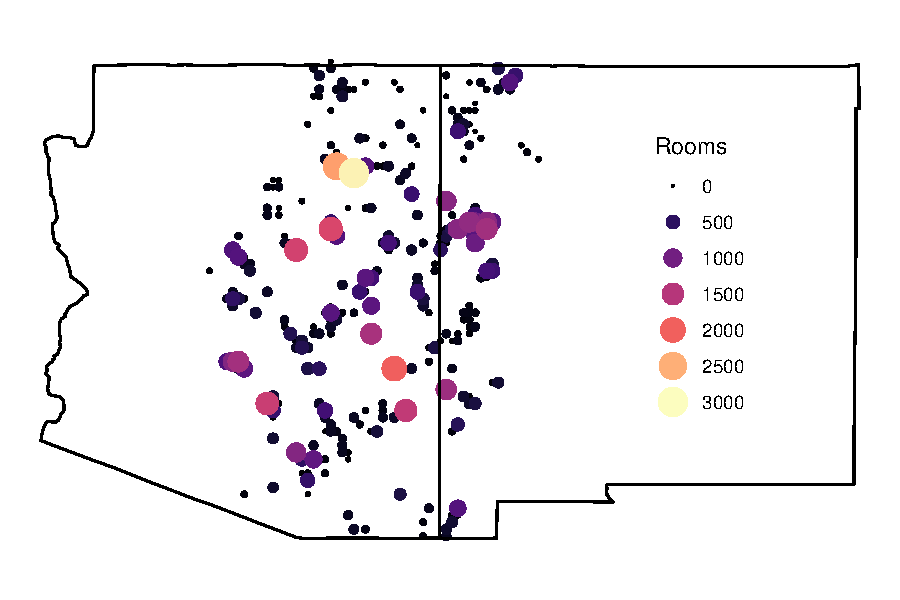
\includegraphics[width=.9\linewidth]{figures/site_distribution.pdf}
\caption{The \emph{Southwest Social Networks} dataset, version 1.} 
%Each line connects a pair of archaeological sites. Line color corresponds to the similarity of the artifact distributions between the pair. A similarity coefficient of 1 means that the sites share the exact same decorated ceramic wares in the exact same proportions, and a coefficient of 0 means there is no overlap in the ceramic assemblages. This similarity network can be interpreted as the degree of social interaction and cultural transmission between sites, whether via migration, trade, or copying. Networks are shown over successive 50 year time spans, starting at 1200 CE. A relatively stable network configuration starting at 1200 CE is interrupted by climatically-forced migrations near the end of the 1250 time step.}
\label{fig:network-plot}
\end{figure}

\section*{Data and Methods}

\subsection*{Hydroclimate Variability}
Climate varies across scales because of many reasons, both dynamic and stochastic, so to understand how droughts impact society we must first separate signal from the climatic noise. To do this, I decomposed a 100-year observational record of summer moisture availability into orthogonal modes of variability, in order to extract the leading patterns that collectively explained the most variability. I analyzed the 100 year dataset of 12 month Standardized Precipitation-Evapotranspiration Index (SPEI) calculated from PRISM data over a domain covering the states of Arizona, New Mexico, Colorado, Utah, and California \parencite{daly}. SPEI is the normalized deviation from the average climate water balance for a given month on varying time scales. I focused on the 12-month SPEI calculated in the August of each year, as agricultural droughts during the summer growing season are most relevant to societies at the time.
%phyda intro?

Principal Components Analysis (PCA) is a common tool for extracting modes of variability in the climate sciences \parencite{lorenz,Hannachi2007}, but has been used only rarely in comparison to archaeological data \parencite{Weiss1982, Cordell2007}. First, I calculated the empirical orthogonal functions (EOFs) via a singular value decomposition of the space time covariance matrix \footnote{This step is equivalent to working on the correlation matrix, as SPEI is already standardized to unit variance at each location.}, multiplying each grid cell by the cosine of latitude to account for areal distortion. Then, I selected the leading eigenvalues for rotation, using both a scree test and North's rule of thumb \parencite{North1982}, which accounts for autocorrelation in the observed data. I rotated the leading eigenvalues using a varimax rotation in order to relax the spatial orthogonality constraints of the EOF analysis and to reveal coherent, physically meaningful patterns \parencite{Richman1986}. The resulting eigenvectors were then multiplied by the square root of the corresponding eigenvalues to yield correlation coefficients and mapped in space. The PC amplitude time series were then compared to the observational record, and the signs of the eigenvalues and vectors were reversed to match the historical record (so that a positive time series value corresponds to a positive SPEI and \textit{vice versa}). In order to show if these patterns are robust over time, the observed EOFs were compared to those calculated reconstructed SPEI values over the last millennium \parencite{Steiger2018}.
%the spatial patterns are the eofs, the time series the PCs

\subsection*{Archaeological Interaction Networks}
(Figure \ref{fig:network-plot}). The Southwest Social Networks (SWSN) database is a compendium of material-culture data from nearly 1,000 well-dated sites in Arizona and western New Mexico from between 1200 and 1500 CE \parencite{Mills2012,Mills2013a,Peeples2013,Borck2015,Hill2015,Mills2015a}. The SWSN project analyzed nearly 4.7 million ceramic artifacts and nearly 5,000 obsidian artifacts \parencite{Mills2015a}. Using an index of the similarity of ceramic assemblages as a proxy for the intensity of social interaction between settlements, the SWSN database provides quantitative estimates of the topology of the region-wide social network during six 50 year time steps \parencite{Mills2013a}. I aggregated the point-based SWSN data into 10km grid cells, so that the results are less sensitive to local settlement dispersal or aggregation \parencite{Paliou2016}, smoothing over the approximate area of each site's resource and raw material catchment \parencite{Varien1999}. Then I calculated a modified Jensen-Shannon divergence between the empirical frequency distributions of 15 decorated ceramic wares at all of the patches
\begin{equation}
    D_{ij} = H\left(\pi_1P + \pi_2Q\right) - \pi_1H(P) - \pi_2H(Q)
\end{equation}
where $D_{ij}$ is the divergence between the empirical frequency distributions of ceramic wares at sites $i$ and $j$, and $H(P) = -\sum_i p_i \ln_2 p_i$ is the Shannon entropy of $H$ measured in bits and $\pi_1 = \pi_2 = 0.5$ are equal weights for the probability distributions. This equation measures the information flow based on the distributions of the ceramic types shared by both sites and the types exclusive to each \parencite{Masucci2011,PaoloMasucci2012}. Analogous to the use of divergence measures in population genetics, divergence here is a proxy for information flow. The index can be loosely interpreted as a probability of interaction between two sites, with identical patterns of ceramic discard indicating a high likelihood of interaction via either direct migration or trade or indirect cultural diffusion.

\subsection*{Least-Cost Networks}
Distance ultimately constrains social interaction, as the further one travels to interact with a partner the greater will be the cost in time, money, and energy. Modelling this spatial structure in the SWSN data is necessary to control for spatial dependence in statistical analyses of these data. To accomplish this, I calculate the least-cost network between all sites in the SWSN network. The topography of the study area was represented using 90m SRTM DEM, resampled to 250m. A cost matrix was calculated containing, for each DEM cell, the amount of time in seconds it would take a hiker to move to each of the 16 neighboring cells. Time costs were calculated using a version of Tobler's hiking function, which estimates walking speed from terrain slope. The function was modified to make it isotropic (i.e. averaging the uphill and downhill walking speeds) and adding an extra penalty to very steep slopes consistent with human cognitive biases. The walking speed values were then converted into absolute time by dividing each pair of neighboring cells by their inter cell distances. This cost matrix (time) was then inverted to represent conductance (speed), facilitating a sparse matrix representation and estimation of least cost paths using efficient graph theoretic algorithms \parencite{Etten2014}. The resulting transition matrix was used to calculate all pairwise isotropic least cost paths between each pair of archaeological sites. 

\subsection*{Spatial Interaction Models}
Spatial interaction models and their variants are used across the social and natural sciences \parencite{Wilson1971,Fotheringham1989,Sen1995,Bavaud2008,Murphy2010,Head2015}. In a regression context, a spatial interaction model estimates the pairwise flow among entities -- resources, migrants, information --  as a multiplicative function of a set of predictor influencing the production and attraction of flows as well as measures of their mutual separation or other generalized costs of moving. Network data representing flows of information and people have several endogenous characteristics that must be correctly modeled in order to make accurate statistical inferences. Spatial interaction models account for this endogenous structure using entropy maximization techniques, which ensure that simulated networks satisfy simple self-consistency constraints, such as that the sum of outflows of from a region is proportional to its inflows. The conceptual justification for the use of spatial interaction models on archaeological networks is directly analogous to that used in molecular ecology \parencite{Murphy2010}, where they are used to estimate flows of information among a spatially-structured metapopulation from the divergences of those populations \parencite{Mesoudi2018}. 

Archaeologists have used statistical spatial interaction models sparingly \parencite{Tobler1971,Hodder1974,Johnson1990ChumashAnalysis} because of the rarity of high-quality archaeological data on social interaction strength \parencite{plogg?}, although the method is seeing a resurgence in simulation studies where data quality is less of a concern \parencite{Bevan2013, Evans2011, Davies2014,Paliou2016}. Archaeological similarity networks have three features that make traditional statistical spatial interaction modeling difficult. These are 1) the data are bounded between 0 and 1, 2) the measures are symmetric 3) we have no exact functional expectations for the specific terms in the spatial interaction model, because empirical work on this scale and type is rare. To address these issues, I used Generalized Additive Models (GAMs) \parencite{Wood2006a}, a semiparametric nonlinear regression technique extending GLMs, to determine whether the patterns of interaction strength from the SWSN database are significantly related to the patterns of variability captured in the EOFs. 

Specifically, I fit models of the form
\begin{equation}
    logit\left(D_{ijt}\right) = f(dist_{ij}) + f_t(EOF_{ij}) + \tau_i + \tau_j + \epsilon_{ij}
\end{equation}
where f() refers to an arbitrary function estimated during model fitting using penalized cubic regression splines, and $\tau_i$ and $\tau_j$ are time-varying random effects for the nodes incident on each edge. The logit function transforms data in the range $[0, 1]$ to $[-\infty, +\infty]$, and also allows the model to be estimated additively. I compared candidate models using AIC, BIC, and $R^2$, and using maximum likelihood, and refit the selected model with REML because of the latter method's better performance. AIC selection between linear mixed models outperformed several other estimating techniques in landscape genetics in simulation studies by \parencite{Shirk2018}. We account for non-independence of observed edges that share origin or destination sites using the maximum likelihood population effects correlation structure, which models the co dependence of errors on shared sites. This helps account for the nature of pairwise data. Pairwise data are high powered, which is why goodness of fit estimates are preferable over statistical significance testing, and we must be careful to properly estimate confidence intervals. 

\section*{Results}

\subsection*{Six drought patterns explain 83\% of observed drought variability in the American Southwest}
The leading 6 PC time series together explain 83\% of the SPEI variance from the 100 year observational record (Figure \ref{fig:scree}). The principal components (PCs) represent SPEI time series that are maximally representative of the entire data set. I rotated the 6 PCs before mapping, in order to capture more physically meaningful patterns and minimize statistical artifacts. PCs beyond the leading 6 were not retained for rotation and mapping, as they represent spatially and temporally incoherent variability and spurious correlations introduced by sampling error in the observational record. 

\begin{figure}[!ht]
\centering
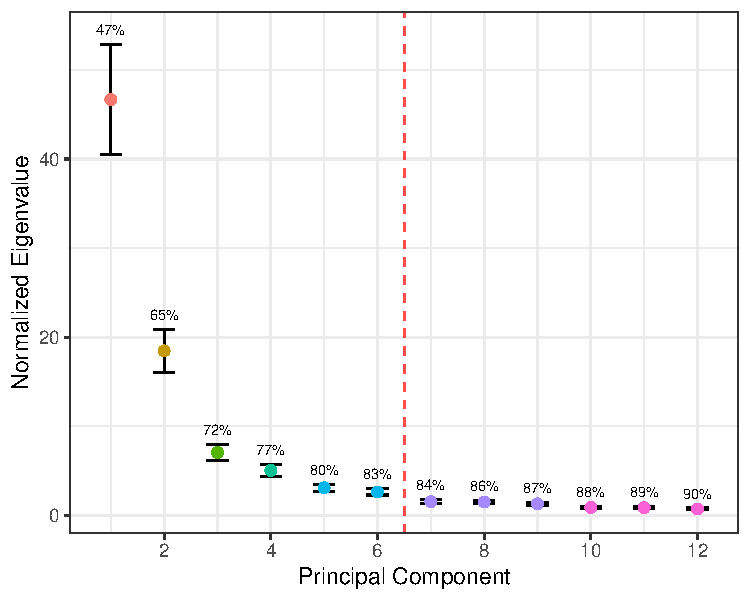
\includegraphics[width=.8\linewidth]{figures/scree.pdf}
\caption{Leading 12 principle components, in order of decreasing eigenvalues, along with the cumulative percent of the variance explained by the leading PCs. Standard errors calculated using North et al.'s rule of thumb \parencite{North1982}. PC's with the same colors (5-6, 7-9, 10-12) are degenerate multiplets, meaning they cannot be clearly distinguished from one another given the sampling variability in the observational dataset. The dashed line represents the truncation point, beyond which PCs were not retained for further analysis. The leading 6 PCs collectively explain 83\% of drought variability in the observed drought record.}
\label{fig:scree}
\end{figure}

\begin{figure*}[!ht]
\centering
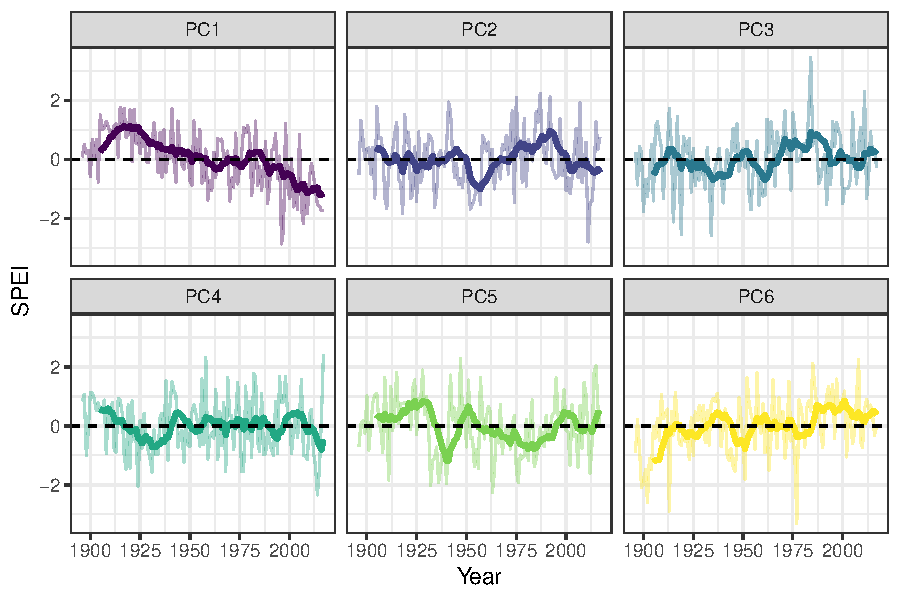
\includegraphics[width=.7\linewidth]{figures/pc_obs.pdf}
\caption{Time series associated with the leading 6 PCs after varimax rotation. SPEI values can be interpreted as z-scores in a normal distribution (i.e. a value of 1 is one standard deviation wetter than average for that location, -1 is one standard deviation drier). The dashed line corresponds to a SPEI value of 0 (i.e. average climatic water balance). 10 year moving averages superimposed over raw annual values. All save PC6 are present in an independent SPEI reconstruction from the last millennium.}
\label{fig:pc-obs}
\end{figure*}

\subsection*{Different drought patterns are associated with different zones of oceanic or continental influence}
To reveal the latent spatial structures associated with the temporal modes of variability, I mapped the spatial patterns associated with each of the leading 6 PCs (Figure \ref{fig:eofs}). The results are robust, recurring patterns of spatially-coherent variability, and can be interpreted as the degree to which 100 year record at each grid cell correlates with the associated rotated PC time series. These spatial patterns are known as the (rotated) empirical orthogonal functions (EOFs). The patterns are consistent regardless of the exact SPEI time scale used to calculate them, which supports their robustness. The spatial and temporal patterns associated with the leading 6 PCs allows us to trace the sources of each mode of variability back to the global climate system.

\begin{figure*}[htbp!]
\centering
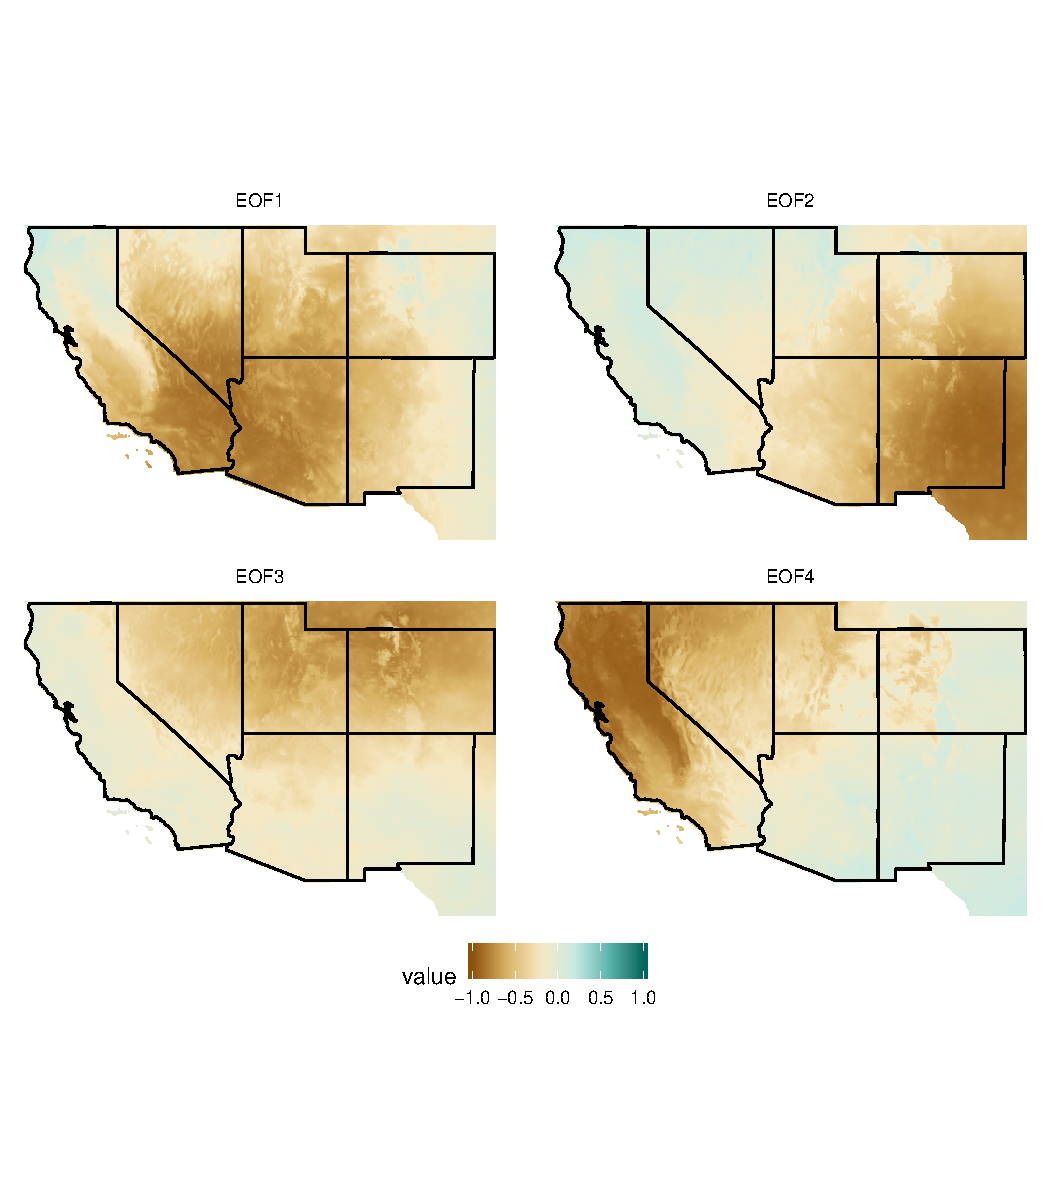
\includegraphics[width=.8\linewidth]{figures/reof_observed.pdf}
\caption{Leading 6 rotated empirical orthogonal functions (EOFs). The empirical orthogonal functions are the spatial patterns associated with their respective principal component time series in Figure \ref{fig:pc-obs}. The EOFs are the eigenvectors of the space-time covariance matrix, and the PCs are the eigenvalues. The leading six EOFs, which together explain 77\% of interannual drought variability in the observational record, were then subjected to varimax rotation, to make the spatial patterns more physically meaningful by relaxing the spatial orthogonality constraint.}
\label{fig:eofs}
\end{figure*}

I diagnosed the dynamic origins of each drought pattern by examining these maps, along with looking at the correlation of the PCs to global sea surface temperature and examining extreme dry and wet periods in each observed PC.
PC1 represents a center of action in the desert Southwest portions of California and Arizona, extending up to the northeast. It represents the influence of tropical Pacific sea surface temperatures, such as the North American Monsoon and tropical storms. This pattern is produced by southwesterly flow from the tropical pacific, bringing moisture up across the low desert zones. The pattern attenuates with gains in elevation, as distance from the ocean increases. PC1 shows an interrupted drying trend to the present day, possibly a global warming trend. PC2 similarly represents southeasterly flow from the Gulf of Mexico, centered eastern New Mexico. As with PC1, the pattern attenuates with increasing elevation and distance from the ocean, due to orographic and continentality effects, respectively. It represents cyclonic storms coming from the Gulf of Mexico, in turn influenced by variability in Atlantic sea surface temperatures. PC2 is the 1950s drought PC2 shows a major dry period centered on the Texas/New Mexico drought of 1956. 

PC3 shows a wet peak in the 1983 Salt Lake City floods, polar continental cold fronts. PC4 clearly represents the influence of westerly flow off the Pacific Ocean, and the orographic effect of the Sierra Nevada mountains intercepting this flow. These include atmospheric rivers (TODO cite uh that paper), and are associated with coastal droughts in California. PC 4 shows dust bowl, and the 1924 drought, reflects California. PCs 5 represent centers of action far removed form the study area. PC5 is centered over the great plains and attenuates across the Rocky Mountains. PC5 is the dust bowl. EOF6 is a round region corresponding with the Colorado Plateau. The mode of variability here is likely temperature dependent, reflecting interactions with radiation at increased elevation. The pattern covaries with elevation, but they are not exact (TODO R2 = ). Variability here is likely linked to Atlantic multidecadal variability. Perhaps the 4 corners high. Arctic oscillation and North Atlantic oscillation for EOF 6. Yes, EOF6 is the AO/NAO, associated with cold dry winters in the west during its positive phase. Consistent with sst correlations and timinng of extreme events (1977). (Myoung et al 2015). PC6 shows up with the 1977 drought in Colorado and California. (TODO) mention sst correlations here too.

%\begin{figure}[!ht]
%\centering
%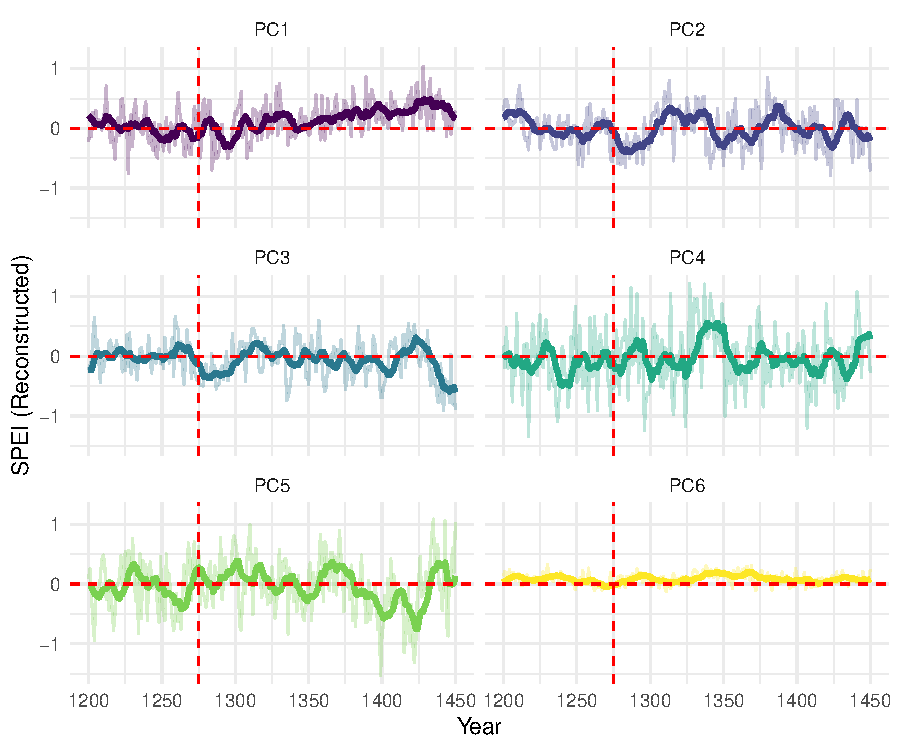
\includegraphics[width=\linewidth]{figures/spei_reconstruction.pdf}
%\caption{}
%\label{fig:spei-reconstruction}
%\end{figure}

\subsection*{Hydroclimate variability explains a moderate but clear proportion of the intensity of social interaction}
The null model for our statistical network analysis was that distance alone accounts for the intensity of social interaction. This null hypothesis, that distance alone is sufficient to explain the observed divergences between archaeological assemblages, was sufficient to explain nearly 35\% of the variance in archaeological dataset. The distance-only model fitted with the exponential deterrence function predicts a rather sharp falloff in interaction at distance (Figure \ref{fig:distance}). As expected, the resulting distance-based network predicts many strong interactions at close distances. This is confirmed by the residuals of the model, which show long distance triangular interactions.

\begin{figure}[!htbp]
\centering
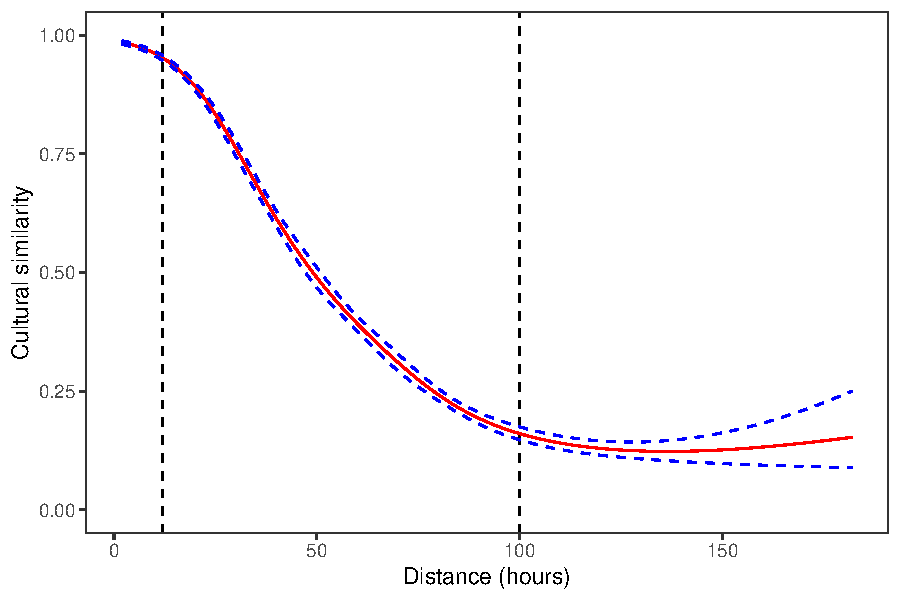
\includegraphics[width=\linewidth]{figures/distance_function.pdf}
\caption{Empirical distance deterrence function.}
\label{fig:distance}
\end{figure}

A model including climatic dissimilarity as a predictor of cultural similarity between all pairs of sites, measured as the absolute difference between their EOF loadings, explains 5\% more variance than the distance-only null model. The increase in variance explained is small relative to the null model but is statistically clear. The model with drought variability also performs better than the null with respect to parsimony and goodness-of-fit. There are three general classes of smooth functions (Figure \ref{fig:smooths}). In many cases, increasing distances along a particular EOF increases the intensity of social interaction, as was expected ahead of time. Just as often, increased distance along a particular EOF has no influence on, or even inhibits, the intensity of social interaction. And finally, the smoothness penalty selects some EOFs out of the model entirely. All functional forms reveal a close to pairwise linear structure in the scale of the linear predictor, with no influence on social interaction between locations with up to 0.2 difference in drought pattern, reflecting the lack of significant distinction between opposing patterns at that scale. 

The intensity of these functional relationships varies smoothly over time. Surprisingly, the waxing and waning of the effect size of a particular EOF has not clear association with the sign of the associated PC amplitude time series reconstructed for each period, suggesting additional dynamic processes are in effect. Rho value of 19\% introduced by nodal covariates, out of a maximum of 50\%. EOF 1 is strongly positive flooding increasing after 1350, corresponding to flooding in the hohokam region, period of high variability in EOF2. Also corresponds to the Salado phenomenon.

\begin{figure*}[!htbp]
\centering
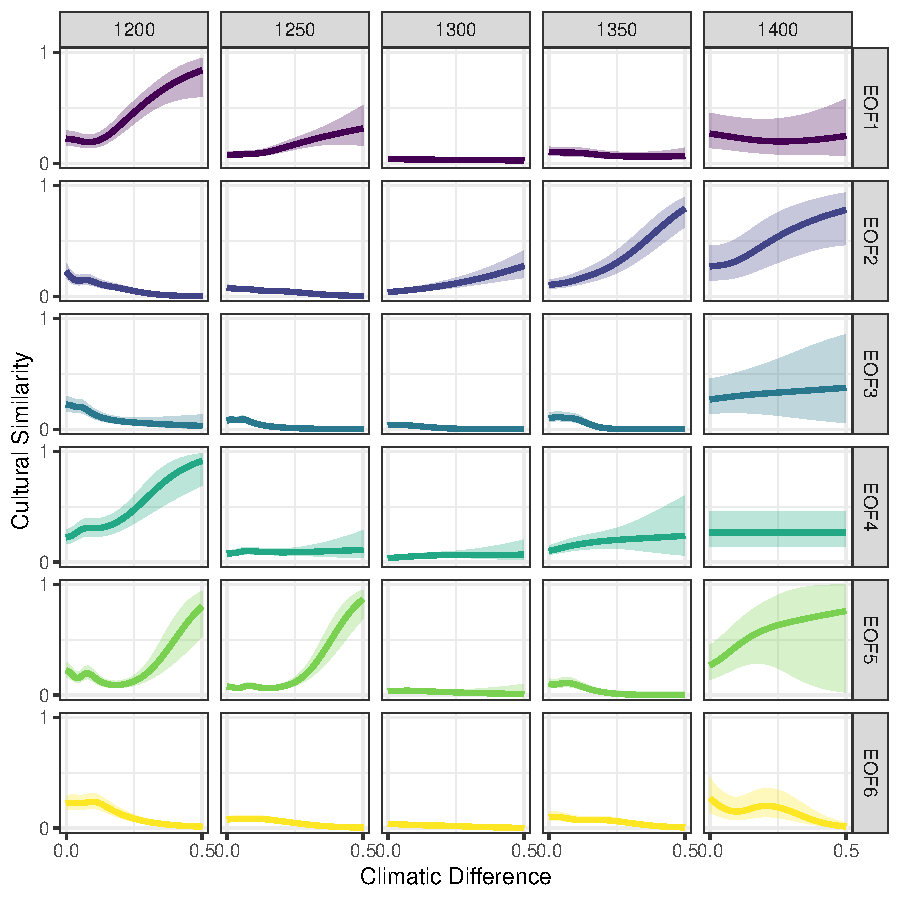
\includegraphics[width=.8\linewidth]{figures/smooths.pdf}
\caption{Estimated smooth functions.}
\label{fig:smooths}
\end{figure*}

\section*{Discussion and Conclusions}
I found 6 spatial drought patterns, each corresponding to a different marine or continental influence. These spatial patterns influenced the flow of social information in different ways -- both enhancing and inhibiting social interaction, and the nature of this effect varies over time. Droughts associated with tropical Pacific and Atlantic influences seem to have been most important for structuring social interaction, with ties connecting these regions greater than chance and distance. These results support and extend previous work in the archaeology and climate of the American Southwest. The intensity of social interaction decays with distance, but increases between regions experiencing different patterns of hydroclimate variability. These results also highlight two more novel points -- the importance of objective, physically-meaningful measures of drought spatial variability and that social interaction dynamics that are out of equilibrium with the biophysical environment environment.

The goal here was to extract robust patterns of climate variability. Measures of point-based sample correlation can easily be dominated by noise or other issues with sampling variability. The method used here yields patterns superficially similar in appearance to point correlations, but in a more objective fashion designed specifically to skillfully extract signal from noise. These patterns represent different zones of moisture transport, reflecting the influence of topography and marine or continental moisture sources \parencite{Liu2010, Hu2011}. These spatial and temporal drought patterns, and their hypothesized forcings from the global climate system, are largely consistent with those from other studies using varied observational data and time windows\parencite{Comrie1999,Cook1999,McCabe1999,McCabe2004,Ryu2010,Seager2014,Herrmann2016}. The spatial patterns are consistent with the general mechanistic understanding of drought variability in the American Southwest: primarily influenced by tropical Pacific sea surface temperatures, additional moisture sources in the North Pacific and Atlantic, and the regional expression of these global influences is in turn mediated by local terrain and atmospheric circulation. These same patterns from the observational period also show up in drought reconstructions spanning the past millennium, emphasizing the fact that these are robust, time invariant spatial modes.

The pair of Pacific and Atlantic SST dominated drought patterns in the Southwest has been previously hypothesized before in the context of archaeological change (dean and van west), but the level of spatial detail here far surpasses previous studies. There in the context of a ``bi-modal precipitation distribution'', meaning the distinguishing between regions with both summer and winter dominate precipitation (PC1) and those with just summer dominant precipitation (PC2). Although specifically growing season (summer) variability is measured here, the pattern is also consistent with winter moisture variability, as the 24 month SPEI index integrates the long lag effects of winter moisture, and the summer and winter patterns are governed by similar atmospheric teleconnections to Pacific SST variability. The strength of the summer monsoon has a strong soil moisture memory effect, and is influenced by the preceding winter's precipitation. The EOF patterns are in part scale dependent. Although the particular choices of variables, resolution, domain size, truncation level, were informed here by theory and tested to as to minimize sensitivity to particular choices made by the authors, different researchers could still generate equally reasonable results given  different input parameters. This is simply to state that the drought patterns highlighted here, while I am confident they are not statistical artifacts, should be used with caution in contexts outside of the specific context here. Our data set is not spatially extensive enough to sample the range of hydroclimate variability. For example, the 5th and 6th EOFs are not greatly expressed in our study area. But there is evidence for long distance exchange between New Mexico and Great Plains cultures \parencite{Spielmann1983} which would be consistent with that pattern influencing exchange. However, given the relative spatial scales of our environmental and cultural data, there is a risk that many different correlated climate patterns will be indistinguishable at the scale of the cultural data. Correlation between competing hypotheses as a source of error in model selection using information criteria \parencite{Shirk2018}.

%zuni and hopi

In spite of the robustness of these spatial patterns, there remains considerable diversity in the functional responses of human social networks to these drought patterns. Based on the risk reduction model we would expect negative homophily on drought regime. Yet, the increased differences in drought regime are just as likely to inhibit social interactions as they are to enhance them. This pattern suggests that climate regimes are serving as a deterrent to social interaction in some way, either as ethnolinguistic divisions or conflict. The evidence for conflict and warfare is equivocal \parencite{Kohler2014, leblanc} but largely points to increased resource variability as a source of conflict. So although drought patterns do influence social interaction, the nature of the interaction varies over time and depends on the specific mode of variability. One explanation is that large scale climate regimes influence ethnolinguistic groups. Save for in boundary zones, small scale quotidian interaction would prefer shared ethnolinguistic affiliation. Interregional exchange may occur higher up a sociopolitical hierarchy, as the flows of goods and information proceeded hierarchically \parencite{Crumley1979}. Perhaps then the strongest signal of interaction is between terminal sites, and takes the form of more elite-focused ceremonial interactions.

Population dynamics in the prehistoric southwest were clearly out of equilibrium \parencite{Hill2004}, not least of which because of the 1275 drought and associated population movements. The spatial interaction model only assumes that the flows are at equilibrium with the population centers, but not that the population centers themselves are at equilibrium. Yet the change of the functional forms for the EOF patterns over time still shows that even these flows point to dynamics occurring longer than our 50 year time scales. Social responses adapted to a particular mode of variability can be fragile to changes in that variability \parencite{Janssen2007}. \textcite{Cordell2007} argue that this pattern breaks down ca 1239-1488, and explain it as the source of disruption in this period as the social networks that developed to cross it over the centuries were not able to adapt in time to the temporarily distinct precipitation regime. -- this is an important point, and why networks aren't always just optimally minimizing correlation, they take time to build and effort to maintain, especially on the time scales greater than a single generation. Free-riding can lead to the breakdown in this critical social infrastructure when it is most needed \parencite{Kohler1996}. So these networks are specifically forming in response to robust patterns of variability. This study sought specifically to investigate the impact of effective distance and drought variability using statistical models, specifically focused on the functional forms of these relationships. Future study will leverage these findings to construct dynamic simulation models. It will be important to model the evolution of paths separately \parencite{Bevan2013} in order to capture this time lag effect. This will allow us to capture year-to-year variability, as well as the time averaging and bias introduced by the use of archaeological similarity data to represent dynamic social processes \parencite{Crema2014}.

%This work says nothing about the role of drought in \textit{producing} similarity, such as a drought leading to many migrants, but rather looks at long term patterns in the costs and benefits of traveling between specific pairs of settlements. This is because I integrate out the mean of each site to get attractiveness, effectively integrating out utility measures \parencite{Bavaud2002,Bavaud2008}. So I am specifically looking at the ``deterrence'' effect of climate distances, that is how climate influences the ``effective distance'' between sites by altering the costs and benefits of interaction.

%There are also different social process at play. Food transfers are thought to have occurred primarily in the context of informal sharing within kin groups, reciprocal exchange at ritual ceremonies and festivals, and residential mobility on the scale of one to three generations \parencite{Hegmon1991,Hegmon1996,Varien1999,Cordell2007,Spiemann1983}.

The residuals from the fitted network models retain unexplained structure. These broadly correspond to large cultural clusters, a common feature in social networks that is not accounted for by either distance or drought variability. On a micro scale, the residuals display a pattern of high transitivity and triad closure, which is to say there are a great many more closed triangle structures than would be expected by chance. Although this feature is common in human social networks, it is also to be expected from the semi-metric nature of the data, as full transitivity is to be expected in a metric with the triangle equality. Kinship, or perceived kinship (ethnicity) important too \parencite{Nolin2010}. The residuals where corresponding to ties that are much less than expected by distance also reveal structure. I see strong directed and spatially discrete clusters of negative interactions that are associated with a pair or few of sites. This may suggest areas of increased conflict, where the kind of social interaction through which pottery would have been exchanged would be rare, or other unmodeled costs of travel such as river crossings cultural taboos. Importance of the ritual contexts of exchange (Plog 19xx, ford 1972). The eof patterns are the selective environment in which norm and institutions regulating social interaction emerge. 

%risks not efficiently pooled \parencite{Fafchamps2007}, dynamics are a reason
These results have utility beyond the prehistoric North American Southwest. They are key for understanding the geography of human adaptation to climate and climate change. These past networks evolved in part in response to robust, time invariant spatial structure. Can we expect certain patterns to change in the future? These findings emphasize the importance of institutional evolution in the developing world, that increases the robustness of human populations to environmental variability.

\printbibliography

\end{document}


